\documentclass[%
aip,
jmp,
amsmath,amssymb,
reprint,
nofootinbib
]{revtex4-1}

\usepackage{graphicx}% Include figure files
\usepackage{dcolumn}% Align table columns on decimal point
\usepackage{bm}% bold math

\begin{document}
	
	\title[Report: Streaming of 3D data]{Streaming of 3D data}
	
	\author{Kevin Hambrecht}
	\author{Sascha Stelling}
	\date{\today}
	
	
	\maketitle
	
	\begin{quotation}
		In this paper we sum up our results of the intern-ship with the Heidelberg Collaboratory for Image processing (HCI)\footnote{\url{https://hci.iwr.uni-heidelberg.de/}}
	\end{quotation}
	
	\section{\label{sec:level1}Summary}
	
	
	
	\subsubsection{\label{sec:level2}Project concept}
	
	Our project is aimed to visualize streaming \\COLLADA\footnote{\url{https://www.khronos.org/collada/}} 3D content. We have a server with the model files stored internally and when a client requests these files, a HTTP multipart stream\footnote{HTTP multipart is part of the HTTP protocol: \\\url{https://www.w3.org/Protocols/rfc1341/7_2_Multipart.html}} is opened to constantly stream the geometry files. With this method, the file on the server may also be a animated geometry, so every stream interval a different model may be streamed which results in an animation being played on the client side. Our project does also support textures, materials and paths for streaming.
	
	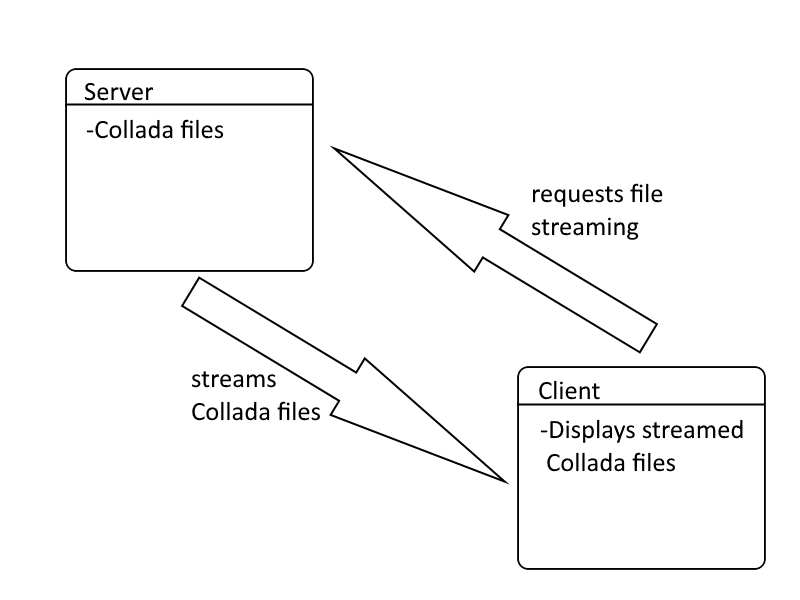
\includegraphics[width=\linewidth]{images/concept}
	
	\section{State of the art of streaming geometry data}
	
	\subsubsection{O3D (open source JavaScript API created by Google, outdated)}
	
	O3D features: Full featured 3D graphics engine which can be downloaded and ran through web browsers. It may load, render and transform models and their respective textures dynamically, using AJAX and/or COMET in real-time. No more traditional compilation of source code is needed, since all necessary ressouces are loaded in real-time
	
	The latest Google Developers Blog post about O3D wrote about a game developer creating a game for social networks using O3D. When going to the developers homepage however, you can see them being closed in 2014.
	
	\subsubsection{SVG (vector graphics file format)}
	
	The Scalable Vector Graphics file format is, as the name implies, used primarily for vector graphics. However, since SVG-files can be modified by scripts that can be loaded on a webpage, it is possible to create 3D animations by transforming the flat 2D paths to the third dimension with such scripts. However, aside from some spinning logos, this method isn't widely used.
	
	For the streaming aspect, there are methods described about how to stream SVG files using HTML like here.
	
	However, SVG isn't used for streaming today and the articles are already more than 2 years old. Also, it is very fiddly to even get a 3D object in SVG and streaming this object has to be done by hand, too.
	
	\subsubsection{VRML(outdated)}
	
	VRML features: Interactive animation, interactive sound, interactive lighting, Streaming is difficult since you would have to download the whole mesh every time. However, there are frameworks trying to solve this problem by creating different LODs (level-of-detail) and a flexible LOD storage scheme
	
	\subsubsection{X3D (Succesor of VRML)}
	
	X3D features: multi-stage rendering, multi-texture rendering, shading with light map and normal map, SSAO, CSM, Realtime Environment Reflection/Lighting
	
	X3D already supports multiple streaming methods which are the following: Anchor, Inline, LOD, LoadSensor, Script and Prototype nodes support successive retrieval of content once initial model is displayed
	
	Currently, there is a french game developing company called 3dduo working on a VR MMORPG with the visualization software BS Contact which is based on X3D. The software page is still up, however, the game homepage only shows a single image.
	
	\subsubsection{X3D vs. Collada}
	
	X3D is only supported by blender and 3DS Max via plugin while Collada is supported by a lot more programs too. However, X3D features programmable shaders, animation, user interaction like dragging and keyboard input, camera movement and linking of objects from different sources. Collada does support animation and programmable shaders, too. The other features that Collada lacks of are mostly easy to implement, eg. for the camera there is already an extension FCOLLADA which offers a variety of camera features.
	
	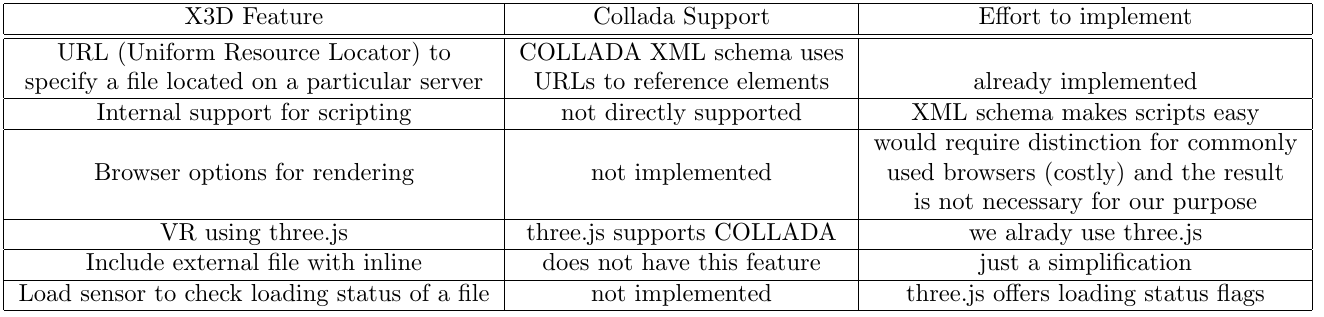
\includegraphics[width=\linewidth]{images/Comparison}
	
	\section{Software we used}
	\subsubsection{The COLLADA file format}
	
	Why did we use COLLADA as geometry file format? COLLADA offers a decent range of tools to display 3D data and its XML-based schema makes it easy to understand and stream. Since it is supported by most common applications it is a great candidate to choose.
	
	\subsubsection{HTTP Multipart streaming}
	The HTTP Multipart protocol is commonly used to upload files to a server or vice versa. To stream a COLLADA file efficiently, we separate the file in different chunks, differentiating between static and dynamic chunks. The static chunks only need to be sent once since they don't change, but the dynamic chunks are to be streamed constantly because they might change any time. For example in our animation a dynamic chink would be the position array and the whole material.
	
	\section{Visualization in the browser}
	
	\section{Finished software}
	
	
\end{document}